%        File: qspn.tex
%     Created: Fri Oct 13 09:00 PM 2006 C
% Last Change: Fri Oct 13 09:00 PM 2006 C
%
\documentclass[a4paper]{article}
\usepackage{color,graphicx}
\usepackage{amsmath}
\usepackage{amsthm}
\usepackage{amssymb}
\usepackage{amsfonts}
\RequirePackage{ifpdf} % running on pdfTeX?
\ifpdf
\usepackage[pdftex,bookmarks=true,
		   bookmarksnumbered=false,
		   bookmarksopen=false,
		   colorlinks=true,
		   linkcolor=webred] {hyperref}
\definecolor{webgreen}{rgb}{0, 0.5, 0} % less intense green
\definecolor{webblue}{rgb}{0, 0, 0.5} % less intense blue
\definecolor{webred}{rgb}{0.5, 0, 0}   % less intense red
\else
\newcommand{\href}[2]{ #1 }
\fi

%%%% Misc
\newcommand{\T}[1]{\textrm{#1}}
\newcommand{\see}[1]{\T{[\ref{#1},pg.\pageref{#1}]}}
\newcommand{\vedi}[1]{\T{vedi \see{#1}}}
\newcommand{\pgra}[1]{\left\{#1\right\}}
\newcommand{\pqua}[1]{\left[#1\right]}
\newcommand{\pton}[1]{\left(#1\right)}
\newcommand{\pass}[1]{\Big|#1\Big|}
\newcommand{\sist}[1]{{ \begin{cases} #1 \end{cases} }}
\newcommand{\eal}[1]{{\begin{align*} #1 \end{align*}}}
\def\ove#1{{\overline{#1}}}
\newcommand{\qq}{\qquad}
%% Defs
\def\*{{\times}}
\def\|{{\;\lor\;}}
\def\&{{\;\land\;}}
\def\-{{\setminus}}
\def\0{{\emptyset}}
\def\8{{\infty}}
\def\v{{\cup}}
\def\^{{\cap}}
\def\<{{\;\Leftarrow\;}}
\def\>{{\;\Rightarrow\;}}
\def\={{\;\Leftrightarrow\;}}
\def\({{\subseteq}}
\def\){{\supseteq}}
\def\'{{\;\;\;}}
\def\,{{,\;}}
\newcommand{\ubrace}[2]{\underbrace{#1}_{#2}}


\title{The QSPN}
\author{AlpT (@freaknet.org)}
\author{http://netsukuku.freaknet.org\\AlpT (@freaknet.org)}
\begin{document}
\maketitle

\begin{abstract}
	This document describes the QSPN, the routing discovery algorithm used
	by Netsukuku.
	Through a deductive analysis, the main properties of the QSPN are
	shown. Moreover, a second version of the algorithm is presented.
\end{abstract}
\pagenumbering{roman}
\pagebreak
\begin{small}
  This document is part of Netsukuku.\\
  Copyright \copyright 2007 Andrea Lo Pumo aka AlpT $<$alpt@freaknet.org$>$.
  All rights reserved.

  This document is free; you can redistribute it and/or modify it
  under the terms of the GNU General Public License as published by
  the Free Software Foundation; either version 2 of the License, or
  (at your option) any later version.

  This document is distributed in the hope that it will be useful, but
  WITHOUT ANY WARRANTY; without even the implied warranty of
  MERCHANTABILITY or FITNESS FOR A PARTICULAR PURPOSE\@.  See the GNU
  General Public License for more details.

  You should have received a copy of the GNU General Public License
  along with this document; if not, write to the Free Software
  Foundation, Inc., 675 Mass Ave, Cambridge, MA 02139, USA.
\end{small}

\clearpage
\tableofcontents
\clearpage
\pagenumbering{arabic}

\section{The general idea}
\label{sec:general_idea}

The aim of Netsukuku is to build a (physical) scalable mesh network, completely
distributed and decentralised, anonymous and autonomous.\\

The software, which must be executed by every node of the net, has to be
unobtrusive. It has to use very few CPU and memory resources. In this way it
will be possible to run it in low-performance machines like Access Points,
embedded devices and old computers.\\

If this requirements are met, Netsukuku can be easily used to build a worldwide
distributed, anonymous and not controlled network, separated from the
Internet, without the support of any servers, ISP's or control authorities.

\subsection{The network model}
\label{sec:net_model}

Netsukuku prioritises the stability and scalability of the net: the network
has to be able to grow to even $2^{2^7}$ nodes.\\

A completely dynamic network would require rapid and frequent updates
of the routes and this is in contrast with the stability and the scalability
requirements of Netsukuku. For this reason, we restrict Netsukuku to the case
where a node won't change its physical location quickly or often.\\

This assumption is licit because the location of a WiFi node mounted on
top of a building won't change and its only dynamic actions would be the
joining and the disconnecting to and from the network and the changes of the
quality of its links.\\

However, there are some consequences with this assumption:
\begin{enumerate}
	\item	Mobiles node aren't supported by Netsukuku algorithms.
		\footnote{It is possible to use other mesh network protocols
		designed for mobility in conjunction with Netsukuku, in the
		same way they are used in conjunction
		with the Internet (i.e. see \href{http://olsrd.org}{olsrd}). }
	\item   The network isn't updated quickly: several minutes may be
		required before all the nodes become aware of a change in the
		network (new nodes have joined, more efficient routes have
		become available, \dots). However, when a node joins
		the network, it can reach all the other nodes from the first
		instant using the routes of its neighbours.
\end{enumerate}

\subsection{The routing algorithm}
One of the most important parts of Netsukuku is the routing discovery
algorithm, which is responsible to find all the most efficient routes of the
network.\\

The routing algorithm must be capable to find the routes without overloading
the network or the nodes' CPU and memory resources.

\subsection{The QSPN}

Netsukuku implements its own algorithm, the \emph{QSPN}.
It is based on the assumptions described in section \ref{sec:net_model}.

\section{Network topology}
\label{sec:net_topology}

The QSPN alone wouldn't be capable of handling the whole network because it
would still require too much memory. For example, even if we store just one
route to reach one node and even if this route costs one byte, we would need
1Gb of memory for a network composed by $10^9$ nodes (the current Internet).\\

For this reason, it's necessary to structure the network in a convenient
topology.

\subsection{Hierarchical topology}
\label{sec:fractal_topology}
Netsukuku adopts a hierarchical structure:
256 nodes are grouped inside a \emph{group node} (gnode), 256 group nodes are grouped
in a single \emph{group of group nodes} (ggnode), 256 group of group nodes are
grouped in a gggnode, and so on. (We won't analyse the topology of Netsukuku. You 
can find more information about it in the proper document: \cite{ntktopology}).\\

Since each gnode acts as a single real node, the QSPN is able to operate independently
on each level of the hierarchy.\\

Since in each level there is a maximum of 256 (g)nodes, the QSPN will
always operate on a maximum of 256 (g)nodes. Therefore we would need just to
be sure that it works as expected on every cases of a graph composed by $\le
256$ nodes. By the way, we'll directly analyse the general case.\\

For the sake of simplicity in this paper, we will assume to operate on level
0 (the level formed by 256 single nodes).

\section{Tracer Packet}
\label{sec:TP}

A \emph{TP} (Tracer Packet) is the fundamental concept on which the QSPN is
based: it's a packet which stores the ID's of the traversed hops in its body.

\subsection{Tracer Packet flood}
\label{sec:TP_flood}

A TP isn't sent to a specific destination but instead, it's used to flood the
network. By saying ``the node A sends a TP'' we mean that ``the node A is
starting a TP flood''.\\

A TP flood passes only once through each node of the net: a node which
receives a TP will forward it to all its neighbours, except the one from which
it received the TP. Once a node has forwarded a TP, it will not forward any
other TP's of the same flood.

\subsection{Properties of the tracer packet}
\label{sec:proprieties_TP}

\begin{enumerate}
	\item A node $D$ which received a TP, can know the exact route covered
		by the TP. Therefore, $D$ can know the route to reach the
		source node $S$ (who sent the TP) and the routes to reach
		the nodes standing in the middle of the route.

		For example, suppose that the TP received by $D$ is: $\left\{
		S, A, B, C, D \right\}$. By looking at the packet, $D$ will
		know that the route to reach $B$ is $C\rightarrow B$, to reach $A$ is
		$C\rightarrow B\rightarrow A$, and finally to reach $S$ is
		$C\rightarrow B\rightarrow A\rightarrow S$.
		The same also applies for all the other nodes which received
		the TP, i.e, $B$ knows that the route to reach $S$ is
		$A\rightarrow S$.
	\item The \emph{bouquet of $S$} is the set of all the TP's which will
		be forwarded or sent by the node $S$ during the flood.
		The first TP of this bouquet received by a generic node $D$,
		will be the TP which covered the fastest route which connects
		$S$ to $D$.
		The fastest $S \rightarrow D$ route is the route with the
		minimum \emph{rtt} (Round-Trip Time) between $S$ and $D$.
		This property is also valid if $S$ is the node which started
		the TP flood, i.e. the first node which sent the first bouquet
		of the TP flood.
\end{enumerate}

\subsubsection*{Example}
\begin{figure}[h]
	\begin{center}
		\includegraphics[scale=0.4]{fig/segABCDEF}
	\end{center}
	\caption{A simple graph}
\end{figure}

Suppose that $D$ sends a TP. The TP will cover the routes:
$D \rightarrow E \rightarrow F$ and $D \rightarrow C \rightarrow B \rightarrow A$.
When the TP reaches the node $F$ and the node $A$, the flood will stop
because either $A$ and $F$ aren't able to forward the TP to any other node.\\

At the end, $A$ will know the route $A \rightarrow B \rightarrow C \rightarrow D$
and $F$ will know the route $F \rightarrow E \rightarrow D$.

\subsection{Acyclic Tracer Packet flood}
\label{sec:acyclic_TP_flood}

The Acyclic flood is not restricted like a normal TP flood: one or more ATP can
pass from the same node. The end of the flood is given by this rule: a node
will not forward the ATP to any of its neighbours if its node ID is already present
in the route contained in the body of the packet. With this rule, an ATP can
walk in a cycle only once, hence the name.\\

Finally, like in the normal TP, a node doesn't forward the ATP to the
neighbour from which it has received the packet itself.\\

If every node of the network sends an ATP flood, then every node will get
all the possible routes to reach any other node.
%%%%TODO%%%%
%The ATP is equivalent to Dijkstra$
%%%%%%%%%%%%

\subsection{Continuous Tracer Packet}
\label{sec:CTP}

A Continuous Tracer Packet (CTP) is an extension of the TP flood: a node will
always forward a TP to all its neighbours, excepting the one from which it has
received the TP.\\

If a node is the extreme of a segment, i.e. a node with just one link, it will
erase the route stored in the body of the TP and will forward back the TP.\\

In short, a CTP is a TP flood that will never end, thus it will continue to
explore all the infinite combination of routes.

\subsection{Interesting Information rule}
\label{intinforule}
This rule can be described in a single phrase:\\

\emph{A Tracer Packet will continue to roam inside}
\emph{the network until it carries interesting information.}
\qq\\

A node considers a received TP interesting when its body contains at least a
new route. In other words, if a TP contains routes already known by the node,
it's considered uninteresting.\\

When a node receives an interesting TP, it forwards the packet to all its
neighbours, excepting the one from which it has received the TP.
If the TP is uninteresting, the packet gets dropped by the node.\\

Note that if a TP is uninteresting for the node $N$, then it is also
uninteresting for all the other nodes. This is because an uninteresting TP
contains routes which has been previously received, memorised and forwarded
by the node $N$. Therefore all the other nodes already know the same
routes too.

\subsubsection*{Example}
\label{sec:cycle_qv2_example}

Consider this graph. \\
\begin{figure}[h]
	\begin{center}
		\includegraphics[scale=0.4]{fig/cycleABC}
	\end{center}
	\caption{The A-B-C-A cycle}
	\label{fig:A-B-C-A}
\end{figure}
Suppose that $A$ sends a CTP. The two CTP's, after having covered the following
two paths will stop:
\[
A \rightarrow B \rightarrow C \rightarrow A \rightarrow B \rightarrow C
\]
\[
A \rightarrow C \rightarrow B\rightarrow A \rightarrow C \rightarrow B
\]
Let's analyze the first CTP step by step, considering that before $A$ sent the
CTP, none of the nodes knew any route.
\begin{description}
	\item[A $\rightarrow$ B] At this point $B$ doesn't know any route to
		reach $A$, therefore it considers this CTP as interesting and
		forwards it to $C$.
	\item[A $\rightarrow$ B $\rightarrow$ C] By looking at this packet, $C$
		learns a route to reach $B$ and $A$.
	\item[A $\rightarrow$ B $\rightarrow$ C $\rightarrow$ A] The node $A$
		learns a route to reach $C$.
	\item[A $\rightarrow$ B $\rightarrow$ C $\rightarrow$ A $\rightarrow$
		B] The node $B$ learns a route to reach $C$.
	\item[A $\rightarrow$ B $\rightarrow$ C $\rightarrow$ A $\rightarrow$
		B $\rightarrow$ C] Finally, $C$ drops the packet because it
		already knows all the routes contained in the CTP.
\end{description}

\section{Network dynamics}
\label{sec:netdyn}
The QSPN v2 defined until now is not suitable for dynamic networks.

\subsection{Extended Tracer Packet}
\label{sec:etp}
The ETP solves the problem of how the graph should be explored and re-explored to
update the maps of the nodes interested in a network change.
It's way of working is based on a simple observation:\\

When a change in the network occurs, only the information stored in the nodes affected by the change must be updated.
The unaffected nodes will still have up to date information that they can simply
redistribute with the use of the Extended Tracer Packets.\\

An ETP is an Acyclic Tracer Packet\footnote{
An ATP (see paragraph \ref{sec:acyclic_TP_flood}) is a normal TP with the following
rule: a node drops the received ATP if its node ID is already present in the route
contained in the body of the packet. Note also, that since it is a normal TP,
it is not reflected back, when it reaches the end of a segment.}
which contains a portion of a map. Since a map is a set of routes and a
route can be described by a TP, the ETP can be considered as different TP's packed together.
Each TP of the ETP is then subjected to the Interesting Information rule (see
\ref{intinforule}).\\

In order to give an exact definition of the ETP, we must examine each case of network change.
\begin{description}
	\item[Changed link]
		\label{ilink}
		Suppose that the quality of the link $A
		\stackrel{l}{\leftrightarrow} B$ changes, (it may improve or get worst).\\
		Let's examine the events starting from $A$, keeping in mind
		that the situation is symmetric for $B$.

		Since the link $l$ changed, it may be the case for $B$ to
		discover new optimal routes.
		For this reason, $A$ will send to $B$ an ETP with all the routes of its
		map, except those of the form $A\rightarrow B\rightarrow \dots$. If $B$ finds
		something interesting, it will forwards the ETP. In detail:
		\begin{enumerate}
			\item $A$ updates its map.
			\item $A$ creates the following set:
			      \eal{
			      &R=\{r\in \ove M\;|\; \T{gw}(r)\neq B\}\\
			      &\T{where: }\\
			      &\qq r\in \ove M \;\= \;r\in M,\;\;  rem(r)=\max \{
			      rem(s)
			      \;|\;s\in M,\;dst(s)=dst(r) \} \\
			      &\qq\T{In other words, $\ove M$ is the set of all the best routes of the map}\\
			      &\qq M \T{ is the set of all the routes of the map of
			      $B$}\\
			      &\qq gw(r)\T{ is the first hop of the route $r$}.\\
			      &\qq dst(r) \T{ is the destination of the route $r$}.\\
			      &\qq \T{rem}(r) \T{ is the Route Efficiency Measure of
			      $r$}.
			      }
			      If $R=\0$ then this algorithm halts.\\
			      Each route $r\in R$ is saved as $(\T{dst}(r), \T{rem}(r))$.
		      \item $A$ creates the ETP:
			\begin{enumerate}
				\item $A$ writes the set $R$ in the ETP.
				\item $A$ appends its node ID, along with the efficiency
					value of the link $l$.
				\item $A$ sets to 1 the \emph{flag of interest}.
			\end{enumerate}
		      \item $A$ sends the ETP to $B$.
		\end{enumerate}
		Suppose the node $C$ has received the ETP from its neighbor
		$N$\footnote{$C$ may be $B$ itself and $N$ may be $A$}.
		$C$ will examine the ETP and, if considered interesting, updates
        its map and forwards the ETP to the other neighbours as
		follow:
		\begin{enumerate}
		\item If the ID of the node $C$ is already present in the
			received ETP, then $C$ immediately drops the ETP and
			skips all the following steps\footnote{This is the acyclic
			rule}.
		\item Let $R$ be the set of routes contained in the
			ETP received by $C$.\\
			Let $M$ be the set of all the routes contained in the map of $C$.\\
		For each route $r\in R$, the node $C$ looks for 
		a route $m\in M$ such that:
		\[\T{dst}(m)=\T{dst}(r),\;\;\T{gw}(m)=N
		\]
		If $m$ exists, then $C$ sets $\T{rem}(m):=\T{rem}(r)$
		\footnote{With this operation, we are actually replacing $m$
		with $r$ in the map $M$}.
		Otherwise $r$ is copied in the temporary set $R'$.\\
		$M$ is sorted, i.e. the routes of the map of $C$ are sorted in
		order of efficiency.
	\item For all $r' \in R'$,
		let $m'\in M$ be a route such that
		$\T{dst}(r')=\T{dst}(m')$. If
		$r'$ is a better alternative to $m'$ and if
		every hop of $r'$ is reachable by $C$,
		then $r'$  is saved in the map of $C$ as the
		tern $(dst(r'), N, rem(r')+rem(C\rightarrow
		N))$. The map is now ordered.
	\item $C$ creates the following set:
		\[
		S=\{s\in \ove M\;|\; \exists r\in R:\;\T{dst}(s)=\T{dst}(r),\;gw(s)\neq N\}
		\]
	\item \label{backpropstep}
		If $S\neq \0$
		\begin{enumerate}
			\item $C$ creates a new ETP, appending the set $S$ and its ID on it.
				The \emph{flag of interest} of this ETP is set to 0. 
			\item The ETP is sent to $N$.\\
				This new ETP will propagate back in the
				same fashion of the previous ETP, i.e.
				until considered interesting. The only difference is when a node
				considers it uninteresting, it just drops\footnote{The node will
				drop the ETP if the \emph{flag of interest} is set to 0 and if it is
				uninteresting} the ETP.
		\end{enumerate}
		The reason for the above procedure is simple: $C$ considers
		uninteresting some of the routes contained in the received
		ETP, then $C$ sends back its better routes which have the same destination of
		those belonging to $R$ (hoping that they will be useful to the
		previous interested nodes).
	\item 	Let \[\ove R=\pgra{r\in R\;|\;\nexists s\in S:\;dst(r)=dst(s)}\] 
		If $\ove R \neq \0$, then the ETP is still interesting: 
		the \emph{flag of interest} remains set to 1.
		$C$ packs the ETP with the set $\ove R$ and adds its ID.
		The ETP is sent to all its neighbours except $N$.\\
		Note \footnote{This step implements the Interesting
		Information rule: only
		good routes are kept, the other are discarded. Notice
		the extension: if the ETP had only one route, it would be
		almost equal to a CTP (the CTP doesn't have the acyclic rule)}
	\end{enumerate}
	The rnodes of $C$ will use the same procedure. In this way, the ETP
	will continue to be propagated until is considered uninteresting.

	\textbf{Observation: }Suppose the following propositions hold:
	\eal{
	&\forall \T{ node }N\;\forall \T{ node }D\;\;
	C_D:= \pgra{\T{route }r\;|\;gw(r)\in V_N,\;dst(r)=D}\\
	&\qq\T{where $V_N$ is the set of all the neighbours of $N$}\\
	&V(C_D):=\pgra{gw(r)\;|\;r\in C_D} \( V_N\\
	&\T{Given } r \in C_D, \T{ let } B(r)\in C_D \T{ such that } 
	rem(B(r))=\max\pgra{rem(s)\;|\;s\in C_D,\;gw(s)=gw(r)}\\
	&\ove {C_D} = \pgra{B(r)\;|\;r\in C_D}\\
	&\forall x\in V(C_D)\;\exists r\in
	\ove{C_D}\^M:\;gw(r)=x\'\'(\gamma)\\
	&\qq\T{where $M$ is the map of $N$}
	}
	If the property $(\gamma)$ holds, then the step \ref{backpropstep}
	can be omitted (in fact, suppose $N$ sends an ETP to $C$ and that $C$
	considers the route $r$ contained in it as uninteresting).\\
	By step \ref{backpropstep}, $C$ sends back to $N$ its known best route
	$s$, with $dst(s)=dst(r),\;rem(s)>rem(r)$. However, $s$ has been
	already sent by $C$ to $N$ (i.e. when the link $N\leftrightarrow C$
	was established), thus by the property $(\gamma)$, $N$ kept memorised
	$s$ in its map $M$. For this reason, the backpropagated ETP doesn't
	bring any new information. If the map described in the topology
	document\cite{ntktopology} is used, then the property $(\gamma)$
	holds.
	
	\item[New link]
	The case where a new link $A \stackrel{l}{\leftrightarrow} B$
	is established is handled  in the same way of the
	\textbf{Changed link} case, because we can consider $l$ as a link with
	a new rem.

	\item[Broken link] \qq\\
		\begin{enumerate}
		\item \label{stepR} $B$ creates the set $R$:
			\eal{
			&R=\pgra{r\in \overline{M}\;|\; gw(r)=A}}
			In other words, 
			$R$ is the set of all the best routes passing through
			$A$. \\
			If $R=\0$ then this algorithm halts.
			
			Each route $r\in R$ is saved as the pair $(\T{dst}(r),
			\T{rem}(r))$.
		\item \label{upmap}
			$B$ updates its map:
			\eal{&\forall r\in M:\;gw(r)=A\;\;\T{ it sets }rem(r):=-\8}
			The routes are then sorted in order of efficiency.
		\item $B$ creates the following set:
			\[
			\ove R = \pgra{r\in \ove M\;|\;\exists s\in R:\;dst(s)=dst(r)}
			\]
		\item $B$ fills the ETP: 
			\begin{enumerate}
				\item $B$ adds in it the set $\ove R$.
				\item $B$ appends its ID.
				\item $B$ sets to 1 the \emph{flag of interest}.
			\end{enumerate}
		\item Finally, $B$ sends the ETP to all its neighbours, except $A$.
		\end{enumerate}
		At this point, the ETP is propagated in the same way of the
		\textbf{Changed link} case.
	\item[A new node joins]
		Suppose the node $A$ is joining the network. It's neighbours
		are $B_1, B_2,\dots, B_n$, which are all already hooked, i.e.
		they aren't joining the net. Then, the \textbf{new link} case is
		applied to each link $A\leftrightarrow B_i,\;\;i=1,2,\dots,n$.
%TODO: a possible improvement?
%		\begin{enumerate}
%			\item Each neighbour $B_i$ sends its whole map to
%				$A$
%			\item $A$ waits until the maps of all its neighbours
%				are received.
%			\item The maps are ``merged'' into a single map, which
%				becomes the map of $A$. In simple words, the
%				merge of two maps result in a map having only the
%				best routes of the two.
%			\item If the neighbours of $A$ are more than one, i.e.
%				$n>1$, then $A$ sends, to each of them, an ETP
%				containing all the primary routes of its
%				map.
%			\item The ETPs are propagated exactly in the same way
%				of the \textbf{worsened link} case (see page
%				\pageref{wlink}).
%		\end{enumerate}
	\item[A node dies]
		When the node $A$ dies, the \textbf{broken link} case is
		simply applied to each link of $A$.
\end{description}

%- joining simultaneo di piu' nodi
%- l'ETP puo' essere spezzettato
%- criptografia dell'ETP
%

\section{QSPN optimisations}
\subsection{Disjoint routes}
The routing table of each node should be differentiated, i.e. it should not
contain redundant routes.\\

For example, consider these $P \rightarrow S$ routes:
\begin{align}
	& PBCFG_1G_2G_3G_4G_5G_6G_7 \dots G_{19} S	\\
	& PRTEG_1G_2G_3G_4G_5G_6G_7 \dots G_{19} S	\\
	& PZXMNO_1O_2O_3O_4O_5S				\\
	& PQPVY_1Y_2Y_3Y_4S
\end{align}
The routes (1) and (2) are almost identical, they only differ only in the first three
hops. On the other hand, the last two are totally different from all the others.\\

Since the first two routes are redundant, the node $P$ should keep in memory only
one of them, saving up space for the others non-redundant routes.
\newline

Keeping redundant routes in the routing table isn't optimal, because if one of the
routes fails, then there's a high probability that all the other redundant
routes will fail too. Moreover, when implementing the multipath routing to load
balance the traffic, there won't be any significative improvements.
\newline

The following distributed mechanism is adopted: 
suppose that the node $N$ receives a generic TP, suppose also that it contains
a route to reach the node $S$. If $N$ considers the TP interesting, then
$N$ will write in the TP the tern $a=(N,S,n+1)$, where
$n$ is the number of routes already known by $N$ to reach the node $S$. In
this way, the other nodes will know that the TP is the $(n+1)-$th route of $N$
to reach $S$.\\

Now suppose that the node $P$ receives the $TP$ (the TP may or may not have passed
through other nodes after having passed from $N$).\\

Let $T_S=\pgra{(a,b,c) \in T \;|\;b=S}$, where $T$ is the set of all the terns
written in the $TP$. $P$ will calculate the following mean:
\[
m=\frac{\sum_{t \in T_S}^{}t_3}{|T_S|}
\]
Where $t_3$ is the third element of the tern $t$ and $|T_S|$ is the number of elements
of the set $|T_s|$.\\ 

The number $m$ indicates how disjoint is the route contained in the $TP$ from
previous routes. If $m\ge 2$, then the route is exactly the copy of a previous
route. If $m\approx 2$, then the route is approximately a copy of a previous
route. If $m=1$, the route is definitely original.\\
%TODO: show a proof ;)
Example: see figure \ref{fig:disjroute}.\\
If $e_r$ is the efficiency of the route $r$, using the value $m$ relative to
$r$, we can obtain a new efficiency value:
\eal{&e_r'=e_r(2-m)k}
Where $k$ is an appropriate positive coefficient. 
The obtained efficiency value $e_r'$ can be used by the $Q^2$ to
decide if the route $r$ is interesting or not.

\begin{figure}[h]
	\begin{center}
		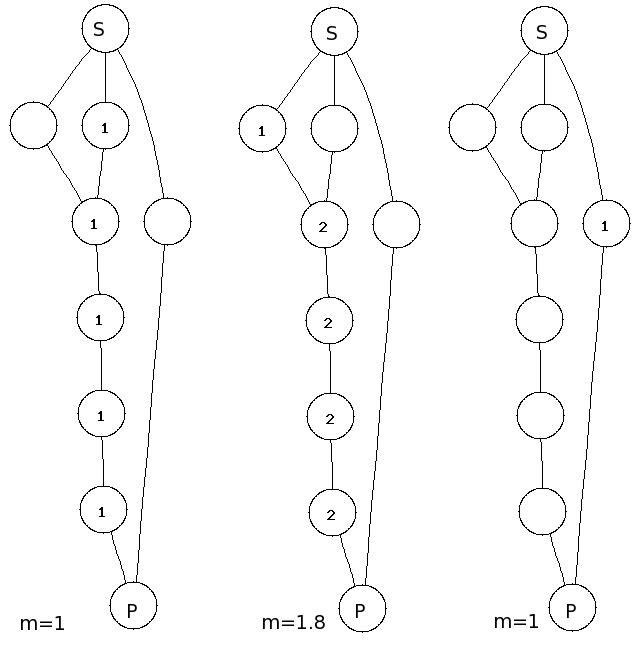
\includegraphics[scale=0.35]{fig/disjrouteU}
	\end{center}
	\caption{Example of the disjoint route mechanism}
	\label{fig:disjroute}
\end{figure}
\pagebreak

\subsection{Cryptographic QSPN}
A node could easily forge a TP, injecting false routes and information about links
in the network. The attack would just create a temporary local damage,
thanks to the distributed nature of the QSPN. However the optimal solution is
to prevent these attacks.\\

Whenever joins Netsukuku, it generates a new RSA key pair. The
continuous generation of keys prevents the leakage of the nodes' anonymity.
The node shares its public key to all the other nodes of its group node.\\
Each entry appended in a TP is then signed with its private key, doing so the
other nodes will be able to prove its authenticity and validate the path
covered by the TP.\\

The size required to store the signatures in the TP can be kept costant using the
aggregate signature system \cite{aggrsign1} \cite{aggrsign2}.

\section{TODO}
\begin{enumerate}
	\item Improve, test and implement the Caustic Routing:
		\href{http://lab.dyne.org/Ntk\_caustic\_routing}{RFC 0013}
	\item Well define a ``secure QSPN''
	\item Research a ``mobile QSPN''
\end{enumerate}

\section{ChangeLog}
\begin{itemize}
	\item \verb|August 2007|
		\begin{enumerate}
%TODO			\item %The ATP is equivalent to Dijkstra
			\item ``Real time issues'' removed from the ETP
				section: it was superfluous.
			\item The whole section regarding the CTP has been
				removed, because until now the ETP is
				sufficient to handle all the routing issues.
			\item An observation regarding the step
				\ref{backpropstep} of the \textbf{changed
				link} case of the ETP has been added.
		\end{enumerate}
	\item \verb|July 2007|
		\begin{enumerate}
			\item The ETP has been simplified: all the cases are 
				now just a minor adaptation of a single case.
			\item Usage of the \emph{tpmask} has been abolished.
			\item Simplified and distributed method to identify
				non disjoint routes.
		\end{enumerate}
	\item \verb|April 2007|
		\begin{itemize}
			\item New section: ``Network dynamics'' (\ref{sec:netdyn})
			\item Description of the ETP (sec.  \ref{sec:etp})
			\item Link ID section remove. With the ETP they are no
				more necessary.
			\item More detailed description of the QSPN v1.
			\item Subsection ``QSPN v2 - High levels'' removed. It
				was redundant with the topology
				document\cite{ntktopology}
		\end{itemize}
	\item \verb|October 2006|\\
		Initial release.
\end{itemize}

%%%%%%%%%%%%%%%%
% Bibliography %
%%%%%%%%%%%%%%%%

\begin{thebibliography}{99}
	\bibitem{ntksite} Netsukuku website:
		\href{http://netsukuku.freaknet.org/}{http://netsukuku.freaknet.org/}
	\bibitem{ntktopology} Netsukuku topology document:
		\href{http://netsukuku.freaknet.org/doc/main\_doc/topology.pdf}{topology.pdf}
	\bibitem{DFS} Depth-First Search:
		\href{http://en.wikipedia.org/wiki/Depth-first\_search}{http://en.wikipedia.org/wiki/Depth-first\_search}
	\bibitem{genrouteawk} Generate Routes in Awk:
		\ifpdf \else \\ \fi
		\href{http://cvs.hinezumi.org/viewcvs/netsukuku/proto/doc/qspn/generate\_routes.awk}{generate\_routes.awk}
	\bibitem{simrouteawk} Simplify Routes in Awk:
		\ifpdf \else \\ \fi
		\href{http://cvs.hinezumi.org/viewcvs/netsukuku/proto/doc/qspn/simplify\_routes.awk}{simplify\_routes.awk}
%%%Obsolete	\bibitem{q2sim} QSPN v2 simulator:
%%%		\ifpdf \else \\ \fi
%%%		\href{http://cvs.hinezumi.org/viewcvs/netsukuku/proto/doc/qspn/q2sim.py}{q2sim.py}
	\bibitem{completegraph} Complete graph:
		\ifpdf \else \\ \fi
		\href{http://mathworld.wolfram.com/CompleteGraph.html}{http://mathworld.wolfram.com/}
	\bibitem{ns2} Network simulator:
		\ifpdf \else \\ \fi
		\href{http://www-mash.cs.berkeley.edu/ns/}{http://www-mash.cs.berkeley.edu/ns/}
	\bibitem{ntkrfc0002} NTK\_RFC 002:
		\href{http://lab.dyne.org/Ntk\_bandwidth\_measurement}{Bandwidth
		measurement}
	\bibitem{aggrsign1}   A Survey of Two Signature Aggregation
		Techniques:
		\ifpdf \else \\ \fi
		\href{http://crypto.stanford.edu/~dabo/abstracts/aggsurvey.html}{http://crypto.stanford.edu/~dabo/abstracts/aggsurvey.html}
	\bibitem{aggrsign2}  Aggregate and Verifiably Encrypted Signatures
		from Bilinear Maps:
		\ifpdf \else \\ \fi
		\href{http://crypto.stanford.edu/~dabo/abstracts/aggreg.html}{http://crypto.stanford.edu/~dabo/abstracts/aggreg.html}

\end{thebibliography}
\newpage

\begin{center}
\verb|^_^|
\end{center}

\end{document}
